\section{Dataset Overview}
\label{sec:eda}

The dataset comprises a total of 50,000 reviews, pre-divided by the dataset authors into 25,000 for training and 25,000 for testing purposes. Each review is assigned a numerical rating ranging from 1 to 10. To simplify the text classification task into a binary feature, the authors suggest a rule: reviews with a score of 4 or below are deemed negative, whereas those with a score of 7 or above are classified as positive. Consequently, reviews with neutral ratings (scores of 5 and 6) were excluded from both the training and test sets. Additionally, both sets are meticulously curated to maintain a balanced distribution of labels, ensuring 12,500 positive and 12,500 negative samples.

To gain insights into the dataset used for training our model, we initiate our exploration by examining basic statistics that offer a comprehensive overview. The primary features of this dataset include the text of the reviews and their corresponding labels. Our focus is on scrutinizing statistics that enhance our understanding of these features, aiming to uncover potential variations based on the labels.


In Figure~\ref{fig:descriptive} we present a summary of our key findings.
In particular, Figure~\ref{fig:labels} confirms the information provided in the dataset description, affirming an equal distribution of reviews between positive and negative sentiments. Figure~\ref{fig:ratings} illustrates the distribution of movie ratings, revealing a fairly symmetric distribution with prominent peaks at extreme ratings (1 and 10), and a relatively uniform distribution across the other ratings. This mirrors the polarized nature of public opinion when evaluating something based on personal preference.

To compute basic statistics on the text, we initiated an initial visual inspection of a sample of reviews. The objective was to discern any patterns that might have influenced the final results. While no significantly influential patterns were observed, a minor issue came to light. Consider the following review:

\begin{quote}
\textit{"All the world's a stage, and its people are actors in it"—or something to that effect. Who proclaimed that theatre ends at the orchestra pit, or even at the theatre door? Why aren't the audience considered participants in the theatrical experience, including the story itself?<br /><br />This film was a grand experiment that declared: "Hey! The story is you, and it requires more than your attention; it demands your active participation." "Sometimes we bring the story to you, sometimes you have to go to the story."<br /><br />Alas, no one paid heed, but that doesn't negate the importance of the message.}
\end{quote}

The review was observed to contain two HTML tags, a pattern observed in numerous reviews within the dataset. Recognizing that these tags may link words, creating a distinctive pattern, we opted to filter them out using a Regular Expression.

Figure~\ref{fig:lengths} provides insights into the lengths of the reviews, indicating negligible differences as the two distributions almost entirely overlap. As a final validation, we examined the potential relationship between review length and ratings, finding no significant differences. As depicted in Figure~\ref{fig:lengths_ratings}, a subtle trend emerges wherein shorter reviews are associated with more extreme ratings. This suggests the possibility that individuals with more pronounced opinions may tend to provide less elaborate arguments. However, it is important to note that we cannot affirm such trends with substantial evidence.

Based on this straightforward statistical analysis, it becomes apparent that there is no significant trend associated with the available features that we can recognize as influential in the classification task. Consequently, our analysis will be conducted solely based on the semantics of the texts.





\begin{figure}
    \centering

    \begin{subfigure}{0.48\textwidth}
        \centering
        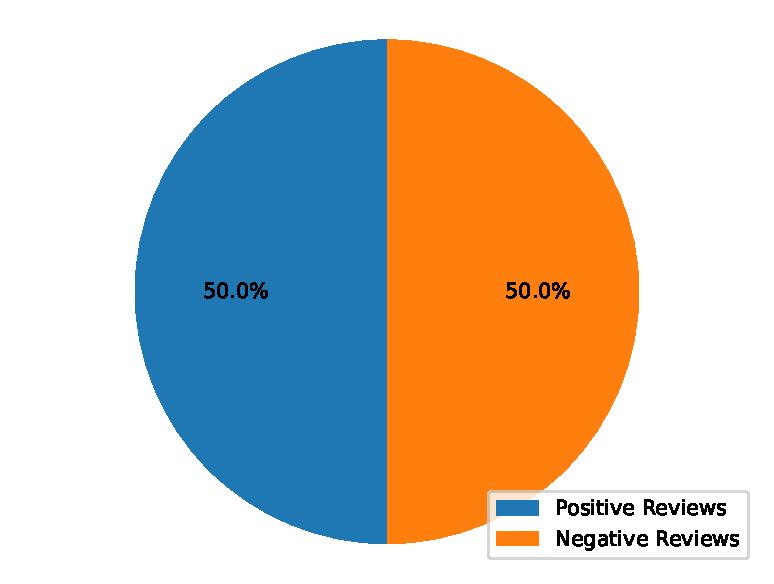
\includegraphics[width=\linewidth]{figures/train_labels.pdf}
        \caption{Distribution of Reviews' Labels}
        \label{fig:labels}
    \end{subfigure}
    %
    \begin{subfigure}{0.48\textwidth}
        \centering
        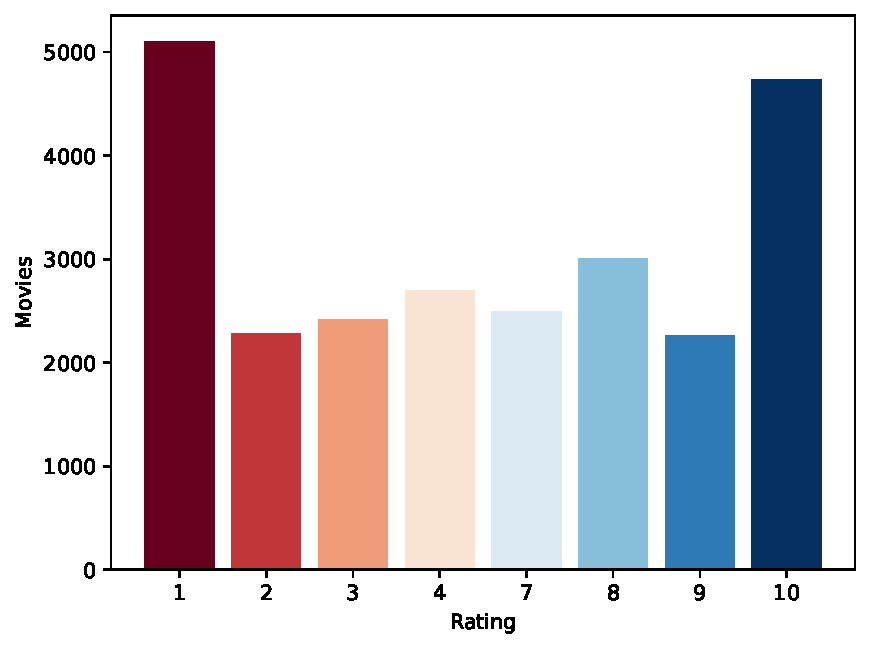
\includegraphics[width=\linewidth]{figures/train_ratings.pdf}
        \caption{Distribution of Movies' Ratings}
        \label{fig:ratings}
    \end{subfigure}

    \vspace{1cm}

    \begin{subfigure}{0.48\textwidth}
        \centering
        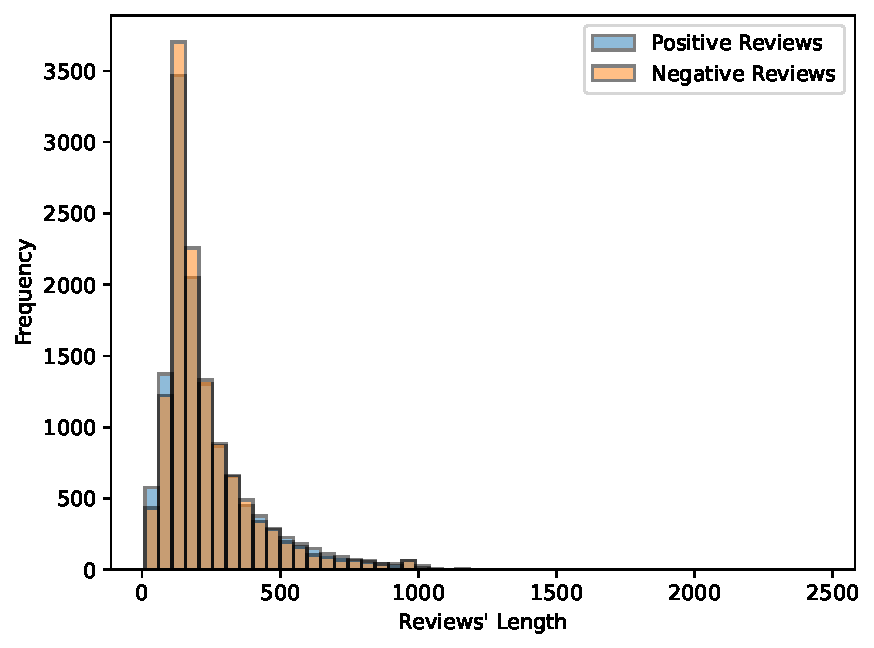
\includegraphics[width=\linewidth]{figures/train_lengths.pdf}
        \caption{Distribution of Reviews' Length (Words)}
        \label{fig:lengths}
    \end{subfigure}
    %
    \begin{subfigure}{0.48\textwidth}
        \centering
        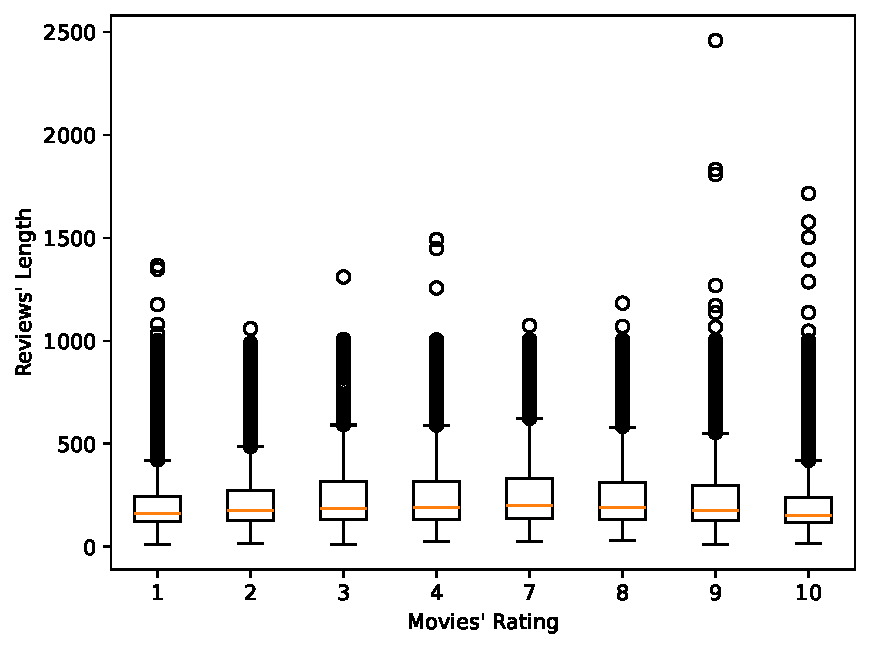
\includegraphics[width=\linewidth]{figures/train_lengths_ratings.pdf}
        \caption{Reviews' Length for Movies' Ratings}
        \label{fig:lengths_ratings}
    \end{subfigure}

    \caption{Exploratory Data Analysis of the IMDb Reviews Movie Dataset \cite{maas2011data}}
    \label{fig:descriptive}
\end{figure}

